%Arik Messerman, September 2006, uidarikmesserman301174 003 0021
%%% KAPITEL 2 ***

\addcontentsline{toc}{chapter}{Hinweise}
\chapter*{Hinweise 1}

%\chapter{Hinweise} \label{kap2}
\section{Verzeichnisse und Nummerierung}
Hier ein kleiner Abschnitt zum Thema Nummerierung von Seitenzahlen, Abbildungen und Tabellen.
\subsection{Seitenzahlen}
Alle Seiten der Arbeit au�er der Titelseite sollten mit einer Seitenzahl versehen sein. Vor dem Beginn des ersten Kapitels werden im Allgemeinen r�mische Ziffern (i, ii, iii, iv, \dots) verwendet. Ab der ersten Seite des ersten Kapitels beginnt die Seitennummerierung neu und l�uft dann bis zur letzten Seite des Dokuments -- einschlie�lich Literaturverzeichnis und eventueller Anh�nge. Daf�r werden dann arabische Ziffern (1, 2, \dots) verwendet. 

\subsection{Abbildungen und Tabellen}
S�mtliche Abbildungen und Tabellen werden durchg�ngig in Abh�ngigkeit der Kapitelnummer nummeriert. Die Nummerierung lautet f�r Abbildungen z. B. \textit{``Abbildung~1.3''}, f�r Tabellen \textit{``Tabelle~2.2''}. Als Beispiele siehe Tabelle \ref{tab:EineTabelle} auf Seite \pageref{tab:EineTabelle} und Abbildung \ref{fig:agent} auf Seite \pageref{fig:agent}.
\begin{figure}[htb]
	\centering
		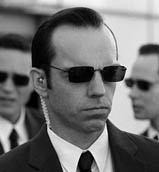
\includegraphics{figures/agent.jpg}
	\caption{Ein Agent}
	\label{fig:agent}
\end{figure}
Auf alle vorkommenden Abbildung und Tabellen muss im Text verwiesen werden. Ist der Inhalt nicht selbsterkl�rend, so sollte auch eine Erl�uterung gegeben werden. \\
Abbildungen oder Tabellen, die gr��er als etwa eine Drittel Seite sind, passen meist besser in den Anhang als in den laufenden Text. 
\begin{table}[ht]
	\centering
\begin{tabular}{||l|r|r|r|r||}
\hline
Verlauf &       2004 &       2005 &       2006 &       2007 \\
\hline
\hline
Deutschland &       2500 &          0 &       5000 &       4500 \\
\hline
   Italien &       1700 &       1000 &       3600 &       5000 \\
\hline
   Schweiz &       2000 &       2000 &       1500 &       2000 \\
\hline
\end{tabular}  

	\caption{Eine Tabelle}
	\label{tab:EineTabelle}
\end{table}
\\
Unter \cite{jam} kann man sich eines Freeware-Tools bedienen, welches die Erzeugung geeigneter \LaTeX -Codes ausgehend aus einer \emph{EXCEL}-Tabelle aus generiert.
\subsection{Inhaltsverzeichnis}
\LaTeX{} erstellt das Inhaltsverzeichnis automatisch aus den Formatvorlagen f�r die verschiedenen �berschriften. Unter Umst�nden ist eine mehrmalige �bersetzung erforderlich damit die Seitenzahlen �bereinstimmen. 

\subsection{Abbildungs- und Tabellenverzeichnis}
L�ngere wissenschaftliche Arbeiten enthalten normalerweise ein Abbildungs- und ein Tabellenverzeichnis. Im Rahmen einer kurzen Seminararbeit kann darauf verzichtet werden.

\section{Fu�noten}
Fu�noten\footnote{Dies ist die eine Fu�note} sollten nur sehr, sehr sparsam verwendet werden. Wenn die amerikanische Zitierweise verwendet wird, die bei der Themenvorstellung erl�utert wurde, kann man eigentlich ganz auf sie verzichten. Wenn unbedingt Fu�noten eingesetzt werden sollen, dann werden sie stets f�r je einen Kapitel fortlaufend mit arabischen Ziffern (1, 2, \dots) nummeriert\footnote{Dies ist weitere Fu�note}.

\section{Literatur und Zitate}
S�mtliche �bernommenen Ideen, Gedankeng�nge oder Formulierung von anderen Autoren m�ssen als Zitate gekennzeichnet werden und eine Quellenangabe gemacht werden. Enth�lt eine Arbeit nicht gekennzeichnete Zitate, so ist sie ein \textbf{Plagiat}. \\
Ins Literaturverzeichnis werden s�mtliche zitierten Quellen aufgenommen. Es werden keine Ver�ffentlichungen angef�hrt, die nicht in der Arbeit verwendet wurden. F�r weitere Hinweise siehe die Pr�sentationsfolien aus der Einf�hrungsveranstaltung.


\section{Layout}
Hier noch die wichtigsten Layout-Parameter:\\
\\
\begin{table}[ht]
	\centering
\begin{tabular}{|l|l|}
\hline
Schriftart/-gr��e: & Times/12pt \\
\hline
Seitenr�nder (oben/unten/innen/au�en): & 2,5/2,0/3,0/2,8 cm \\
\hline
Zeilenabstand: &    Einfach \\
\hline
Absatzabstand: &        6pt \\
\hline
\end{tabular}  
	\caption{Layout-Parameter}
	\label{tab:layout}
\end{table}
\\